% Main article.
\documentclass[futureinternet,article,submit,moreauthors,pdftex]{Definitions/mdpi}
\usepackage{adjustbox}
% Back-matter command compatibility with the bundled MDPI class.
\providecommand{\institutionalreview}[1]{\par\vspace{6pt}\noindent{\fontsize{9}{9}\selectfont\textbf{Institutional Review Board Statement:} #1\par}}
\providecommand{\informedconsent}[1]{\par\vspace{6pt}\noindent{\fontsize{9}{9}\selectfont\textbf{Informed Consent Statement:} #1\par}}
\providecommand{\dataavailability}[1]{\par\vspace{6pt}\noindent{\fontsize{9}{9}\selectfont\textbf{Data Availability Statement:} #1\par}}
\firstpage{1}
\makeatletter
\setcounter{page}{\@firstpage}
\makeatother
\pubvolume{1}
\issuenum{1}
\articlenumber{1}
\pubyear{2026}
\copyrightyear{2026}
\history{}
\Title{Audit Feedback, Decisions, and Explanations in LLM Trading Agents}
\newcommand{\orcidauthorA}{0009-0006-3974-5490}
\newcommand{\orcidauthorB}{0000-0002-9155-269X}
\Author{Aldan Jay $^{1,}$*\orcidA{} and Rafael Berlanga $^{2}$\orcidB{}}
\AuthorNames{Aldan Jay, Rafael Berlanga}
\address{%
$^{1}$ \quad Escola de Doctorat, Universitat Jaume I, Castell\'o de la Plana, Spain; jay@uji.es\\
$^{2}$ \quad Universitat Jaume I, Castell\'o de la Plana, Spain; berlanga@uji.es}
\corres{Correspondence: jay@uji.es}

\abstract{We ask whether audit feedback changes large language model agents' actions or only their explanations. This matters for oversight of autonomous agents in networked services. An earlier exploratory phase motivated our preregistered comparison of five audit conditions in a simulated market with a known, switching return driver. DeepSeek is primary; Haiku and Luna are replications. We reverse a market signal and repeat the prompt to test whether the action changes, then compare this dependence with stated reasons. In DeepSeek, false auditor labels (placebo) shifted decisions toward the false feature more than explanations acknowledged (strategic-compliance index, SCI \texorpdfstring{$= -0.134$}{= -0.134}, Holm \texorpdfstring{$p < 0.001$}{p < 0.001}). Evidence feedback reduced reliance on the true driver (\texorpdfstring{$-0.062$}{-0.062}, Holm \texorpdfstring{$p = 0.014$}{p = 0.014}); Luna replicated this effect. DeepSeek showed no reliable change in explanation precision. Correct labels gave no evidence that explanations changed more than decisions. Haiku showed no effect after correction, and the false-label effect did not generalize across both replications. Contrasts estimate whole audit packages. The instrument passed the pooled check only; it discriminated poorly in one market regime for two models. These findings identify neither internal reasoning nor intent. Oversight interfaces should assess decisions and explanations together.}
\keyword{large language models; explanation faithfulness; counterfactual attribution; accountability; auditing; agent-based simulation; intelligent agents; multi-agent systems; autonomous agents; human--AI oversight interfaces}
\reftitle{References}
\newcommand{\Fprobe}{\mathcal{F}}
\newcommand{\ind}{\mathbf{1}}
\begin{document}

\section{Introduction}
Large language model (LLM) agents increasingly act autonomously in networked services and online markets. Examples include trading and e-commerce agents connected through APIs, as well as multi-agent platforms. In these intelligent-agent systems, remote oversight can use logged explanations and automated auditor services. These services form an intelligent human--computer interface between agents and human or automated supervisors. Explanations communicate reasons, and auditor feedback can steer later behaviour. Explanation evaluation is therefore part of designing oversight channels for Internet applications and smart systems. Our controlled simulation examines this feedback relationship. It does not evaluate a network deployment, communication protocol, or networking performance.

An auditor may accept an agent's explanation without knowing whether the stated reasons influenced its action. This problem arises when large language models (LLMs) select actions in decision-support and agentic systems. Users may trust an output because of its explanation. Auditors or operators may also use that explanation to decide whether to intervene. In the European Union, Article 13 of Regulation (EU) 2024/1689, the Artificial Intelligence Act, requires high-risk AI systems to provide sufficient transparency for deployers to interpret their outputs and use them appropriately~\cite{ai_act_2024}. Explanations therefore need evidential value. Our synthetic trading task is not a legal compliance assessment or a claim that every trading application falls within that provision.

An explanation can agree with an evaluator yet say little about the accompanying action. Generated rationales can omit influential factors~\cite{turpin2023}. Research on self-generated counterfactual explanations and decision explanations raises related concerns~\cite{wang2025,lee2026}. The evaluator may also supply the expected answer. Agreement can then reflect adoption of an authoritative label. We test whether the associated decision changes as well.

Our preregistered confirmatory experiment uses a controlled market. The fundamental component of returns depends on news or momentum and switches repeatedly between them. Agents observe these features, trade, and cite their reasons. We measure two kinds of agreement. \emph{Environmental fidelity} means that an agent cites the feature currently driving fundamental returns. \emph{Restricted process alignment} means that cited features agree with features whose sign reversal changes the agent's action. To measure it, we use a \emph{counterfactual sign-flip probe}: we reverse one feature's sign, keep the rest of the prompt fixed, and re-ask for an action. Environmental fidelity concerns the environment. Restricted process alignment concerns the agent's response to this intervention. Neither measure provides direct access to internal reasoning.

An earlier exploratory phase used a different and weaker design: it measured environmental fidelity only, used nearly identical agents and a different set of conditions, and revised its hypotheses after a pilot. It found that agents cited any label the auditor disclosed, even a false one. Its apparent fidelity gain under corrective audits became inconclusive once decisions exposed to disclosed labels were excluded. We call this pattern auditor echo. It motivated the present preregistered experiment, which measures decisions as well as explanations. Preliminary data are never pooled with confirmatory data and provide no confirmatory evidence.

We therefore distinguish citation adoption from decision sensitivity under institutional feedback. Following that exploratory motivation, we test whether auditor echo extends to decisions. In DeepSeek, the placebo audit package increased opposite-driver sign-flip dependence more than citation relative to naive under the registered SCI. The evidence audit package also reduced true-driver sign-flip sensitivity relative to naive in the primary model and one replication. Neither comparison isolates feedback content from auditing and fines. We report null results, contrary effects, instrument weaknesses, and model differences alongside these findings.

\subsection{Background and related work}\label{sec:related}
\paragraph{Explainable AI and explanation faithfulness.}
Research distinguishes models that people can interpret from post hoc explanations, which are generated after a prediction~\cite{rudin2019}. Other work examines what interpretability means~\cite{lipton2018} and surveys explanation methods~\cite{guidotti2018,samek2021,barredo2020}. Social and pragmatic accounts ask what explanations are for and how to evaluate them~\cite{miller2019,paez2019}. Local surrogates such as LIME approximate a prediction near one input~\cite{ribeiro2016}. Additive attribution methods such as SHAP divide a prediction among input features under particular assumptions~\cite{lundberg2017}. Generated rationales require separate evaluation. Chain-of-thought explanations can omit experimentally introduced influences~\cite{turpin2023}, and a model's own counterfactual account need not locate its decision boundary~\cite{wang2025}. Jacovi and Goldberg distinguish faithfulness, or accuracy about the basis for a decision, from plausibility to a reader~\cite{jacovi2020}. We use this distinction to report environmental agreement and behavioral-probe agreement separately.

\paragraph{Counterfactual measurement of process alignment.}
A model can propose a counterfactual explanation without anyone changing its input. Our counterfactual experiment instead holds the decision context fixed and re-queries the action after reversing one feature's sign. The measured change is a property of the model--prompt--provider system under that intervention. It does not fully decompose the causes of the decision. Correlated features, interactions, unprobed inputs, response variability, and altered input plausibility can still affect the result. Our precision and recall therefore cover only the two probed features. The explanation--behavior gap is a behavioral index, not a report of hidden computation.

\paragraph{LLM agents in markets and strategic settings.}
LLM market simulations study financial behavior~\cite{chen2025}, and market games examine bounded strategic reasoning~\cite{evans2023}. Stylized facts are recurring statistical patterns in empirical returns~\cite{cont2001}. They can validate realistic finance simulations, whereas our market prioritizes controlled fundamental-return generation. Generative agents also operate in interactive social environments~\cite{park2023}. Related work addresses double-auction collusion~\cite{collusion2025}, strategic communication and information leakage~\cite{snake2026}, and adversarial coordination~\cite{byzantine2026}. We examine how institutional messages relate to declared reasons and measured decision sensitivity. We do not aim for trading realism or infer strategic intent.

\paragraph{Auditing, transparency, and accountability.}
Work on the limits of transparency~\cite{ananny2018}, legal debates about explanation~\cite{wachter2017}, and ethical frameworks for AI~\cite{floridi2018} warns against equating disclosure with understanding. Internal auditing frameworks~\cite{raji2020} and recursive audit architectures~\cite{triagent2025} provide institutional context. Cheap-talk theory~\cite{crawford1982} and narrative economics~\cite{shiller2019} help frame why messages may matter, although our study does not test those theories directly. The confirmatory phase compares feedback that names a driver with feedback that reports observational evidence. Neither kind is assumed to equal independent verification by a human institution.

\section{Materials and Methods}\label{sec:methods}
\subsection{Study design}
The confirmatory experiment compares five feedback conditions in a simulated market. The primary model is \texttt{deepseek-v4-flash} (DeepSeek), run with twenty paired market seeds (200--219). Two independent replications use \texttt{anthropic/claude-haiku-5.5} (Haiku) and \texttt{openai/gpt-6-luna} (Luna) with ten seeds each (200--209). Every seed is crossed with all five conditions, so conditions are compared within seeds. Development seeds (100--101) are excluded. Each run has six agents trading for forty ticks. Seeds, not decisions or agents, are the replication units. The primary analysis window is ticks 20--39, which contains two regime switches; ticks 10--39 form a fixed sensitivity window. Figure~\ref{fig:design} summarizes the design.

\begin{figure}[tbp]
\centering
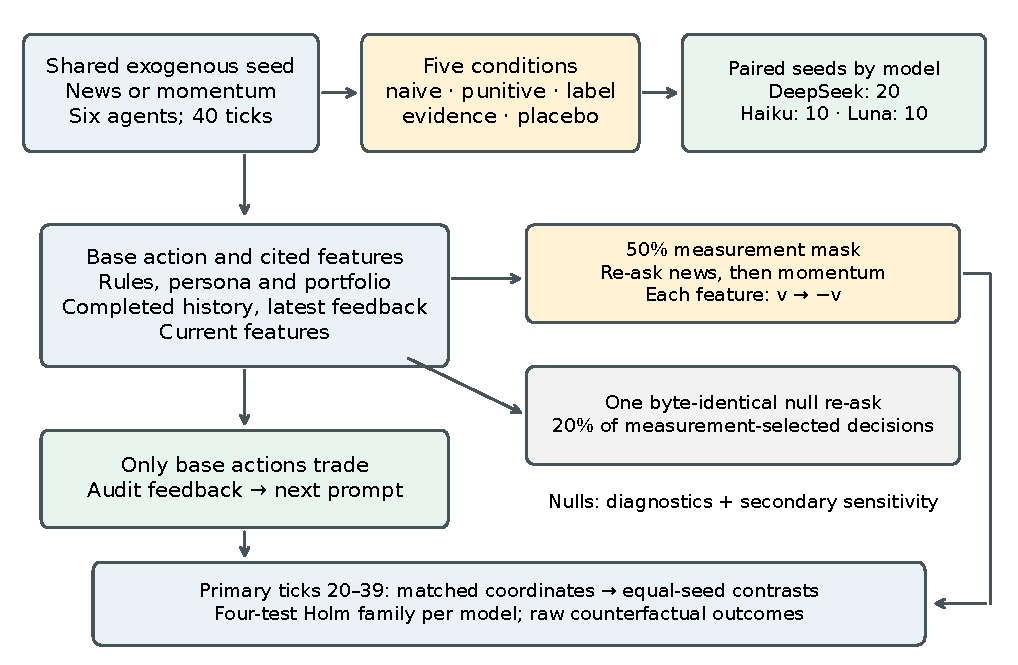
\includegraphics[width=.92\linewidth]{figures/fig1_design.pdf}
\caption{Confirmatory design. Conditions share the exogenous random draws of each seed. Only base decisions trade; sign-flip and null re-asks reuse the base context and never execute trades. The null re-ask rate is the amended design; its realized sampling recipe deviated as reported in Section~\ref{sec:limitations}.}
\label{fig:design}
\end{figure}

\subsection{Market and agents}
The market has one asset. Each return combines the active driver, order imbalance, and noise. Let $g_t\in\{\mathrm{news},\mathrm{momentum}\}$ be the active fundamental driver and $x_{g_t,t}$ its observed value. With $s_{it}=\pm1$ for buy/sell and requested size $q_{it}$,
\begin{equation}
 I_t=\frac{\sum_{i=1}^{N}s_{it}q_{it}}{5N},\qquad
 r_t=0.02\,x_{g_t,t}+0.03\,I_t+\epsilon_t,\qquad
 \epsilon_t\sim\mathcal{N}(0,0.005^2),\qquad
 P_{t+1}=\max\{50,P_t(1+r_t)\},
 \label{eq:market}
\end{equation}
with $N=6$ and $P_0=100$. A latent standard-normal signal plus noise (standard deviation 0.7) forms the active feature; the inactive one is pure noise. Four distractors (spread, volume, orderflow, sentiment) are generated independently, and orderflow and sentiment correlate weakly with momentum and news. Even seeds start in the news regime and odd seeds in momentum; regimes switch at ticks 10, 20, and 30. Agent orders therefore change later prices and observed histories, so treatment effects include these feedback paths.

Agents combine three risk mandates (cautious, balanced, growth) with two starting portfolios (4000 cash units and 20 asset units, or 1000 and 50), all worth 6000 at the initial price. Assignments are identical across seeds, conditions, and models. Each prompt contains the institutional rules, the agent's mandate and portfolio, the latest audit feedback, four completed feature--return rows, and the current features. Agents must answer in strict JSON with a buy or sell action, an integer size from 1 to 10, and up to two reasons chosen from the six features. There is no hold option, and borrowing and short selling are not allowed. Model reasoning output is disabled. The rule text is identical across conditions except for one sentence describing the feedback; the verbatim prompts are part of the preregistration in the public repository.

\subsection{Feedback conditions}
In every audited condition, each decision is audited with probability 0.30 against the current driver (Table~\ref{tab:conditions}). An explanation passes if its reasons include that driver. A failed audit costs 10\% of total wealth (cash plus marked position value). Feedback appears in the next prompt and persists until the next audit, including across regime switches, so a correct label can become stale and a placebo label can become correct.

\begin{table}[tbp]
\caption{Feedback conditions. All conditions require explanations and share the same institutional text.}
\label{tab:conditions}
\centering\footnotesize
\begin{tabular}{llp{.6\linewidth}}
\toprule
Condition & Audit rate & Feedback after an audit \\
\midrule
naive & 0 & None \\
punitive & 0.30 & Pass/fail verdict and the fine, if any \\
label & 0.30 & Verdict and fine, plus the true driver at the audited tick \\
evidence & 0.30 & Verdict and fine, plus correlations of all six features with returns over the last eight ticks; no driver named \\
placebo & 0.30 & Truth-based verdict and fine, plus the opposite (false) driver \\
\bottomrule
\end{tabular}
\end{table}

These conditions are packages. The evidence condition adds a longer history and correlations that include price impact from agent orders, so it does not isolate numerical presentation. The placebo condition combines a correct verdict with a false label, so it does not isolate label falsity.

\subsection{Counterfactual sign-flip probe and metrics}
A prespecified random mask, shared across conditions, selects half of the decisions for measurement. For each valid selected decision we re-ask twice with the exact same context, once replacing the current news value $v$ by $-v$ and once doing the same for momentum. A random 20\% of these decisions also receive one byte-identical null re-ask, which measures response variability. Re-asks never trade.

For decision $j$, let $a_j$ be the base action, $a_j^{(f)}$ the action after reversing feature $f$, $R_j$ the cited reasons, $g_j$ the current driver, and $\Fprobe=\{\mathrm{news},\mathrm{momentum}\}$. We define
\begin{equation}
 E_j=\ind[g_j\in R_j],\quad d_{jf}=\ind[a_j^{(f)}\ne a_j],\quad
 P_j=\frac{|C_j\cap D_j|}{|C_j|},\quad Q_j=\frac{|C_j\cap D_j|}{|D_j|},
 \label{eq:metrics}
\end{equation}
where $C_j=R_j\cap\Fprobe$ are the cited probe features and $D_j=\{f\in\Fprobe:d_{jf}=1\}$ the features whose reversal changes the action. $E_j$ is environmental fidelity, $d_{j,g_j}$ is true-driver dependence, and $P_j$ and $Q_j$ are process precision and recall. Precision and recall are undefined when their denominator is empty and cover only the two probed features; they measure agreement with this probe, not access to internal reasoning.

The strategic-compliance index (SCI) compares how much citation of a feature changes with how much decisions come to depend on it. For seed $s$, condition $c$, naive reference $n$, matched eligible decisions $J_{sc}$, and target feature $X_j$,
\begin{equation}
 \mathrm{SCI}_s(c;X)=\frac{1}{|J_{sc}|}\sum_{j\in J_{sc}}\Big[\big(\ind[X_j\in R_{cj}]-\ind[X_j\in R_{nj}]\big)-\big(d_{cj,X_j}-d_{nj,X_j}\big)\Big].
 \label{eq:sci}
\end{equation}
A positive SCI means that citation rose more than measured dependence, the predicted signature of explanation-only adaptation. A negative SCI means that dependence rose more. Label SCI targets the current true driver and placebo SCI its opposite at every primary-window decision, regardless of exposure (an intention-to-treat selector). SCI is an operational behavioural index; its sign does not identify intent or deception.

\subsection{Hypotheses and statistical analysis}
The preregistered hypotheses predicted positive effects: evidence would raise process precision and true-driver dependence relative to naive (H1); label would raise environmental fidelity and precision (H2); label would show a positive SCI, i.e., strategic compliance (H3); placebo would show a positive SCI, more false citation, and lower fidelity than label (H4); and punitive feedback would gain less precision than evidence (H5).

The primary family has four contrasts for each model: P1, evidence minus naive precision; P2, evidence minus naive true-driver dependence; P3, label SCI; and P4, placebo SCI. Each uses a two-sided paired $t$ test over seed-level differences, with equal seed weights and common eligible decisions. Holm correction is applied within each model; models are not pooled, and replications cannot rescue a failed primary prediction. We report the mean difference $\Delta$, $d_z$ (mean over standard deviation of seed differences), and descriptive 95\% bootstrap intervals from 10{,}000 paired-seed resamples. At 80\% power and the strictest Holm threshold, the minimum detectable effects were $d_z=0.81$ with 20 seeds and $d_z=1.28$ with 10. Registered sensitivities use sign-flip permutation tests, seed-clustered regressions with a wild bootstrap, and the wider window. Invalid responses count as missing and are never replaced by fabricated actions.

\subsection{Preregistration, calibration, and amendments}
The plan was preregistered and frozen before confirmatory data collection; the frozen plan, its amendments, and its checksum are in the public repository. The original probe set features to adversarial extremes. In the development pilot it saturated: DeepSeek changed its action in 109 of 114 true-driver probes (0.956), above the preregistered 0.95 ceiling, and non-driver probes flipped almost as often. Amendment~1 replaced it, before any confirmatory data, with sign reversal. The choice followed a rule fixed in advance on development seeds: among zeroing, sign reversal, one- and two-standard-deviation shifts, and the original extremes, choose the perturbation that maximized the smallest true-minus-non-driver flip-rate difference across models, subject to naive true-driver rates between 0.10 and 0.90. Sign reversal was selected (smallest difference 0.184). Development null re-asks gave response-variability rates of 4--5\%. Amendment~1 also added null monitoring and fixed the provider routes below. The authors had seen descriptive development outcomes for the label condition before freezing; hypotheses, contrasts, windows, and thresholds were not changed. Amendment~2, made during collection, changed only a spending threshold.

\subsection{Models and data collection}
DeepSeek ran through its own API at temperature zero. Haiku and Luna ran through OpenRouter, pinned to their original providers without fallback. Their endpoints did not support a temperature setting, so they used provider-default sampling. Transient transport failures were retried with identical payloads, and valid responses were never resampled. Exclusive locks and a check of the frozen plan's checksum protected collection.

\section{Results}\label{sec:results}
\subsection{Primary contrasts}
All 200 assigned runs completed, with no replaced seeds: 100 for DeepSeek and 50 each for Haiku and Luna. Invalid base responses numbered 0, 6, and 3, respectively, and every primary contrast retained all seed pairs. Table~\ref{tab:primary} reports all registered contrasts.

\begin{table}[tbp]
\caption{Registered primary contrasts. P1: evidence minus naive precision; P2: evidence minus naive true-driver dependence; P3: label SCI; P4: placebo SCI. All predicted signs were positive. Intervals are descriptive 95\% paired-seed bootstrap intervals; Holm correction is within each model.}
\label{tab:primary}
\centering\footnotesize
\setlength{\tabcolsep}{4pt}
\begin{adjustbox}{max width=\linewidth}
\begin{tabular}{llrrlrrr}
\toprule
Model & Test & $n$ & $\Delta$ & 95\% interval & Raw $p$ & Holm $p$ & $d_z$ \\
\midrule
DeepSeek & P1 & 20 & -0.0137 & [-0.0431, 0.0140] & 0.3683 & 0.3683 & -0.2061 \\
DeepSeek & P2 & 20 & -0.0624 & [-0.0981, -0.0239] & 0.0047 & 0.0140 & -0.7164 \\
DeepSeek & P3 & 20 & -0.0389 & [-0.0881, 0.0068] & 0.1364 & 0.2727 & -0.3478 \\
DeepSeek & P4 & 20 & -0.1341 & [-0.1772, -0.0916] & \(1.04\times10^{-5}\) & \(4.18\times10^{-5}\) & -1.3257 \\
\midrule
Haiku & P1 & 10 & 0.0163 & [-0.0362, 0.0642] & 0.5613 & 1.0000 & 0.1907 \\
Haiku & P2 & 10 & -0.0059 & [-0.0609, 0.0531] & 0.8499 & 1.0000 & -0.0616 \\
Haiku & P3 & 10 & -0.0354 & [-0.0892, 0.0210] & 0.2542 & 0.7625 & -0.3852 \\
Haiku & P4 & 10 & -0.0572 & [-0.1045, -0.0039] & 0.0666 & 0.2666 & -0.6596 \\
\midrule
Luna & P1 & 10 & -0.1198 & [-0.1562, -0.0838] & 0.0002 & 0.0007 & -1.9472 \\
Luna & P2 & 10 & -0.0909 & [-0.1396, -0.0312] & 0.0125 & 0.0376 & -0.9832 \\
Luna & P3 & 10 & -0.0333 & [-0.0845, 0.0252] & 0.2883 & 0.2883 & -0.3568 \\
Luna & P4 & 10 & 0.0404 & [-0.0069, 0.0821] & 0.1272 & 0.2544 & 0.5314 \\
\bottomrule
\end{tabular}
\end{adjustbox}
\end{table}

Every DeepSeek primary estimate pointed opposite to its prediction. Evidence precision (P1) and label SCI (P3) were inconclusive. Evidence feedback reduced true-driver dependence (P2), and placebo SCI was negative (P4); both remained significant after Holm correction, in the direction opposite to prediction. Inconclusive contrasts do not establish the absence of an effect.

Figure~\ref{fig:decomposition} splits each SCI into its citation and dependence components. Under correct labels, DeepSeek cited the true driver more often, but its decisions came to depend on that driver even more. Under false labels, citation of the false feature rose, and dependence on it rose about twice as much. Correct labels therefore gave no evidence of explanation-only adaptation, and false labels moved decisions more than the explanations acknowledged.

\begin{figure}[tbp]
\centering
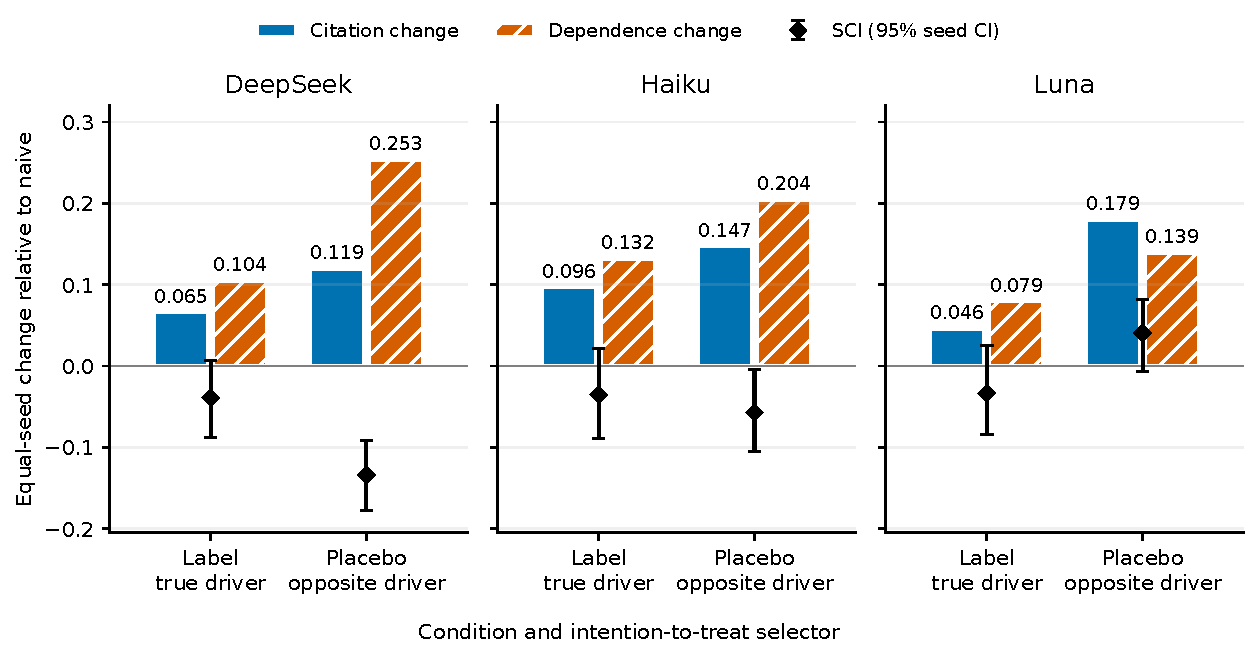
\includegraphics[width=.92\linewidth]{figures/fig3_sci_decomposition.pdf}
\caption{SCI decomposition on matched primary-window decisions, with equal seed weights. Bars show the change in citation and in dependence relative to naive; diamonds show their difference (SCI) with a descriptive 95\% seed-bootstrap interval. Label targets the current true driver and placebo its opposite, regardless of audit exposure.}
\label{fig:decomposition}
\end{figure}

\subsection{Replications and hypothesis verdicts}
Neither replication supported a predicted positive effect. Haiku had no contrast that survived correction. Luna replicated the evidence effect on true-driver dependence and also showed lower precision, while both of its SCI tests were inconclusive. Haiku's placebo SCI was negative but not significant, and Luna's was positive and not significant, so the DeepSeek placebo result did not generalize across models. Table~\ref{tab:verdicts} gives the preregistered verdicts for the primary model.

\begin{table}[tbp]
\caption{Preregistered hypothesis verdicts for DeepSeek. Secondary components use descriptive intervals and carry no confirmatory rejection rule.}
\label{tab:verdicts}
\centering\footnotesize
\begin{tabular}{>{\raggedright\arraybackslash}p{.2\linewidth}>{\raggedright\arraybackslash}p{.18\linewidth}>{\raggedright\arraybackslash}p{.52\linewidth}}
\toprule
Hypothesis & Verdict & Basis \\
\midrule
H1 evidence & not supported & P1 negative and inconclusive; P2 significantly negative \\
H2 label & mixed & Fidelity and true-driver citation rise; precision does not \\
H3 strategic compliance & not supported & P3 negative and inconclusive \\
H4 false authority & mixed & P4 significantly negative, contrary to prediction; false citation rises and fidelity falls below label, as predicted \\
H5 punishment & secondary direction observed & Evidence exceeds punitive in precision, but punitive is below naive; not confirmatory \\
\bottomrule
\end{tabular}
\end{table}

\subsection{Instrument validity and response noise}
In naive, sign reversal of the true driver changed the action in about half of the probes (DeepSeek 0.563, Haiku 0.497, Luna 0.552), within the preregistered 0.10--0.90 range, and more often than reversal of the non-driver (differences 0.201, 0.185, and 0.198). This pooled check passed in every model, but the regimes differ. In the news regime, the difference reversed for DeepSeek ($-0.116$) and was near zero for Haiku (0.003); it was positive in the momentum regime for both and in both regimes for Luna. In these strata, flips indicate sensitivity to the sign reversal rather than correct use of the driver. All strata remain in the registered tests.

Identical-prompt null re-asks changed the action in 2--9\% of cases, depending on model and condition. DeepSeek did so even at temperature zero. Primary outcomes use raw flips, which therefore combine intervention effects with this response variability.

\subsection{Sensitivity, secondary, and exploratory analyses}
Permutation tests, seed-clustered regressions, and wild-bootstrap tests kept every primary sign and agreed with the paired tests at the 0.05 level. In the wider window, two raw decisions changed (DeepSeek P1 and Haiku P4), both remaining negative. Agents adopted disclosed labels heavily: DeepSeek cited the disclosed label in more than 99\% of exposed prompts, whether the label was true or false. Evidence exceeded punitive feedback in DeepSeek precision, but punitive was below naive, so this does not show a benefit of evidence over no audit.

We also ran analyses that were not preregistered. Compared with the punitive condition, which shares the verdicts and fines, evidence still had lower true-driver dependence in all three models, most clearly in DeepSeek. The DeepSeek P2 and P4 directions held in both regimes and after subtracting each seed's null-flip rate. Luna's placebo SCI, by contrast, had opposite signs in the two regimes, and after noise adjustment the descriptive interval of DeepSeek's label SCI fell below zero. These analyses describe robustness and heterogeneity; they do not replace any registered verdict. All secondary and exploratory estimates are available in the repository.

\section{Discussion}\label{sec:discussion}
\subsection{What an auditor's agreement establishes}
Agreement with an auditor does not show what controlled an action. Environmental fidelity alone cannot establish that relationship. Under the registered sign-reversal instrument, the label and placebo audit packages change measured sign-flip sensitivity and citations relative to naive. Correct-label SCI provides no evidence of disproportionate citation improvement in any model. Inconclusive tests cannot exclude all explanation-only changes. The principal placebo-package result is narrower. DeepSeek's negative SCI indicates that the increase in opposite-driver sign-flip dependence exceeded the increase in opposite-driver citation under the registered SCI. The gap is defined relative to naive and does not mean that explanations never mention the false feature.

Oversight should assess environmental agreement and behavioral alignment separately. An auditor can change the system it evaluates. Its message is therefore an intervention as well as a measurement. Audits should test message accuracy, including stale and incorrect feedback, alongside whether the agent repeats the correct answer. The Article 13 motivation is methodological: information supplied for interpretation should have an evidential basis. This experiment does not establish a legal sufficiency test or a complete operational audit standard.

For networked auditing services, feedback channels should be evaluated as interventions and as records of oversight. An apparently authoritative message may steer an autonomous agent's decisions even when its label is incorrect. Matching an auditor's vocabulary is therefore insufficient evidence that an oversight interface supports reliable supervision. Evaluations of multi-agent systems should distinguish explanation agreement from decision sensitivity. They should test stale or erroneous feedback alongside accurate messages. These design implications for intelligent agents and human--AI oversight interfaces are subject to the instrument and model limitations reported here. The experiment establishes neither deployment safety nor the effectiveness of a particular network architecture.

\subsection{False-authority risk}
The placebo audit package can change decisions and citations, but this experiment cannot isolate why. The intervention combines an environmental verdict with a conflicting authoritative driver label. Its effects could reflect message salience, ambiguity resolution, or reliance on the disclosed feature. Under the registered SCI, the placebo package increased opposite-driver sign-flip dependence more than citation relative to naive in DeepSeek. These two response rates are not calibrated measurements of a common latent quantity. Salience, response variability, fixed-history inconsistency, or citation-format constraints could contribute. The result motivates testing responses to erroneous authority. It does not establish under-explanation, concealment, or a mechanism attributable to label falsity alone.

The model differences constrain this result. Haiku's placebo estimate is negative but fails its corrected primary test. Luna's is positive and inconclusive. The DeepSeek result therefore does not establish how LLMs generally respond to audits. Persisted labels and the deliberate verdict/label inconsistency also differ from many practical audits. These features make false authority testable here while limiting direct deployment generalization.

\subsection{Why numerical evidence may hurt}
The evidence audit package did not yield the predicted gains in registered process measures. The evidence condition had lower true-driver dependence than naive in DeepSeek and Luna. The registered comparison does not isolate the effect of its correlation table from audits and fines. Luna precision was also lower, while Haiku remained inconclusive. Instrument checks passed the pooled flip-rate gate only. Precision/recall measures agreement with the probe rather than ground-truth process accuracy. Exploratory evidence-minus-punitive dependence estimates remain negative. Their intervals are descriptive, and the history/content difference is not isolated. Several explanations remain compatible with the design. Short-window correlations can be noisy. The evidence window can span a regime switch, and observed returns contain order imbalance influenced by agent orders. A table over every feature may distribute attention toward distractors or preserve an outdated association. Its longer summarized history also changes information availability rather than presentation alone. Future factorial tests could examine these interpretations; they are not established mediators.

Lower dependence does not automatically imply poorer economic performance. The true feature governs only the fundamental return component. Appropriate trading can also depend on portfolio constraints or impact. The observed decreases concern the registered sign-flip-sensitivity/precision targets in this setting. Reversed or absent discrimination precludes describing every decrease as poorer driver use. Evidence has a relative precision advantage over punitive in DeepSeek, but it does not show an advantage over naive.

\subsection{Limitations}\label{sec:limitations}
The market is synthetic and deliberately simple. News and momentum are generated variables, and a known switch schedule governs the fundamental component. Forced buy/sell choices can elicit decisions when evidence is weak. Short horizons and an oracle environmental auditor that knows the true driver limit resemblance to real markets. Treatment changes market paths through agent orders. A paired seed controls externally generated draws but does not isolate a direct linguistic mechanism. We tested only three deployed models and one prompt family. We did not use immutable checkpoints or broad prompt/order counterbalancing.

The instrument probes only news and momentum. It holds history and correlated distractors fixed and records action rather than size. Sign reversal avoids the original adversarial extremes but can still produce an unusual combination of features and context. The probe can miss interactions, asymmetric thresholds, correlated predictors, and altered confidence without an action change. Sensitivity does not show that a feature was necessary or capture complete process faithfulness. Passing the pooled flip-rate gate does not remedy the news-regime discrimination reversal in DeepSeek or near-zero discrimination in Haiku. Exploratory regime strata preserve the negative DeepSeek P2/P4 directions in both regimes but reveal opposing Luna P4 signs. These exploratory results narrow the interpretation rather than validate the instrument. We therefore cannot interpret every flip as correct use of the environmental driver.

Null re-asks reveal response variability, including with DeepSeek temperature zero. Haiku and Luna used provider-default sampling without temperature control. Rate subtraction is a secondary additive sensitivity. It does not correct individual decisions. It also does not use deconvolution, a method for separating signal from noise statistically. The paired noise sensitivity resamples seed-level rates and contrasts together. All-tick cell subtraction cannot eliminate time/regime heterogeneity or estimate a pure feature effect. Model-by-condition noise differences and the disclosed null-mask/invalid-base deviations complicate that interpretation. Provider-default replication sampling also prevents attributing cross-model differences to model identity alone. Precision and recall have treatment-dependent undefined denominators. Common support reduces comparability problems without making the quantity being estimated unconditional. The gap can reflect either component. Its sign does not identify internal reasoning or intent, and it cannot establish deception.

Development calibration and noise checks reused dev seeds. The authors also saw descriptive label outcomes before freezing. The amendments transparently preserve the original plan and hypotheses. They do not erase that exposure or make instrument choice independent of the development context. The second amendment occurred during collection and was restricted to costs and operations. Two implementation deviations affected only null monitoring: null re-asks were sampled with a slightly different random recipe than registered, and one invalid Haiku decision received a null call; neither changes the primary outcomes. Future preregistered work should validate instruments across regimes and prompt families before testing treatment effects.

Fixed personas and inventory differences do not make six independent decision makers. Within-run dependence remains. Seed counts limit sensitivity to small effects. The two replications have fewer seeds than the primary model cohort. An inconclusive contrast is not equivalence. A positive or negative SCI is an operational behavioral comparison, not evidence for a human motivational category.

\section{Conclusions}\label{sec:conclusions}
The confirmatory experiment shows why explanation change and decision change must be measured separately. The earlier exploratory phase provided motivation only. All four primary DeepSeek estimates oppose their predicted positive directions. The evidence-dependence effect and placebo SCI reject after correction in directions opposite to prediction. Evidence precision and label SCI remain inconclusive.

The evidence condition also reduces true-driver sign-flip dependence relative to naive in Luna, while Haiku has no corrected primary rejection. This estimates an audit package, not isolated numerical content. In DeepSeek's placebo condition, the increase in opposite-driver sign-flip dependence exceeded the increase in opposite-driver citation under the registered SCI. This is also a package contrast. The negative gap does not generalize across both replications. It does not establish explanation incompleteness or deceptive intent. Exploratory regime and paired noise analyses preserve the main DeepSeek directions but reveal heterogeneous Luna SCI and sensitivity of label SCI to noise adjustment. No registered conclusion is replaced. Auditor agreement is insufficient evidence of process alignment, and the evidence package is not automatically beneficial. Evaluation should distinguish environmental agreement, intervention-defined dependence, coverage, noise, and incorrect-authority responses while respecting the limits of the probe.

\vspace{6pt}
\authorcontributions{Conceptualization, A.J.; methodology, A.J. and R.B.; software, A.J.; validation, A.J.; formal analysis, A.J.; investigation, A.J.; resources, R.B.; data curation, A.J.; writing---original draft preparation, A.J.; writing---review and editing, A.J. and R.B.; visualization, A.J.; supervision, R.B.; project administration, A.J. All authors have read and agreed to the published version of the manuscript.}
\funding{This research received no external funding.}
\institutionalreview{Not applicable. The study involved no human participants or animals; all experimental subjects were automated language-model agents accessed through public APIs.}
\informedconsent{Not applicable.}
\dataavailability{All code, data, the preregistration with its amendments and freeze record, and analysis outputs are available at https://github.com/AldanJJay/audit-feedback-llm-agents (preregistration: preregistration/preregistration.md; frozen plan SHA-256: dd8eaf872b37593433b3168725962937394d1b5d1c4ef005fe415534c37235a1, recorded in preregistration/FROZEN.json; interpretive report: results/confirmatory\_results.md; raw data in data/ and code in src/).}
\acknowledgments{The authors thank the developers of the open-source tools used in this work. Use of AI-assisted tools is described in the statement below.}
\conflictsofinterest{The authors declare no conflicts of interest.}
\vspace{6pt}\noindent{\fontsize{9}{10}\selectfont\textbf{Use of Artificial Intelligence:} During the preparation of this work, the authors used AI-based tools to support software development, data analysis, and the drafting and editing of the manuscript. The authors reviewed and edited all outputs and take full responsibility for the content of this publication.\par}

\bibliography{references}
\end{document}
